\chapter{Discussion}\label{chap:Discussion}

Here we present hypothesis and thoughts on different aspects of the simulations and results. 

Most sections describe themes primarily related to simulation. Otherwise all sections state their relevance in the beginning.

\section{Demand Balancing}

Due to the limited number of action the demand has to be matched to fit the pump flows. If this matching is not done nearly perfect results are diverging. An unbalanced demand, means large periods of the demand are greater or smaller than the highest or lowest pump flow respectively. Without randomness reinforcement learning handles the imbalance, it essentially requires that you always follow the best actions. Without grasping the full context or reasoning to this problem, randomness sometimes results in an action which starts a loop of bad actions, resulting in divergence. From many hours of simulation, heuristic evidence, show balancing demands make the algorithm much more robust toward randomness.

In the results shown in \cref{chap:Simulation} and \cref{chap:Results} the pump flow are:

\begin{equation*}
	q(k)=
	\begin{bmatrix}
		6 &  8 & 10
	\end{bmatrix}l/min
q(k)=\{6\;\; 8 \;\; 10\}
\end{equation*}

and the demand flows are:

\begin{equation*}
	d(k)\in [5.44,\; 9.9] \; l/min
\end{equation*}


 A potential solution could be to add more pumps to the pumping station, which would result in more actions and a better coverage of varying demand profiles. This in turn increases the size of the table in tabular Q-learning and adds extra weight vectors in function approximation Q-learning with discrete actions. 
With perspective to the real world, where additional pumps come at a cost, and demands cannot be controlled. The option of running 0 pumps should be included and pumps should be slightly too powerful equivalent to demands being balanced slightly too low.

\section{Hyper Parameters}
As mentioned previously sweeping hyper parameters sequentially is not ideal. In future work these sweeps should be performed more thoroughly by evaluating combinations of parameters. Any change of one hyper parameter changes the optimal selection of the other parameters. This could not be done within the scope of this project, due to coding- and simulation time required to obtain the results. 

The \textit{tendencies} that are often refereed to in sweeping results are subject to randomness, especially for the height approximation method. In reference to the \textit{law of large numbers} tendencies would require a large amount of simulation before being applicable. Results in this project are simulated multiple times, but not enough. This induces some ambiguity in the results of the sweeps. In future work, the ideal sweep incorporates both combinations of parameters and satisfy the law of large numbers.

In a thorough sweep we also suggest considering the convergence of Q values as an evaluation metric. We have not used this method enough to express its advantages, but there seem to be useful information to be achieved in addition to moving average cost evaluation.

Finally a few thoughts on the \textit{cutoff} and its implementation. The cutoff was used in this project as an evaluation tool, but could be implemented by reducing $\epsilon$ and $\alpha$ either after a threshold or continuously. This would unlock the optimal behaviour, instead of adding some suboptimal behaviour from learning and exploration. If changes to the environment are expected, these parameters could be increased to detect and learn these changes, and then reduced back to cutoff values, continuing optimal behaviour.

\section{Premature Convergence}
The tabular method show the ability to converge without exploring the entire state space. This is against expectations, but we present a two part explanation. First we place emphasis on the oscillating demand, which allows the algorithm to see a specific state multiple times without knowing how to \textit{stay} in that state. Secondly each time a state is seen, the algorithm gets one step closer to learn the optimal action in that step. We will consider the scenario where ascending states are explored, heading toward the top of the reservoir. As we explore the \textit{0 cost} area of the barrier function, the only cost assigned to a state is primarily from the action (flow) itself, and the pressure induced from reservoir water level \ref{eq:WDN_Power}. As the tank level increases, the difference between the action cost increments increases, and this difference increases a lot more when the barrier is hit. When the difference in increments are big enough, the algorithm will choose the lower action increasingly many times in a row before the cost has incremented far enough that its cost is higher than another action's. Eventually, the number of \textit{low-flow} actions in a row, will result in the water level decreasing further than what is expected from the demand at that time. This unexpected decrease results in the algorithm seeing a state that it has already fully learned, and it will deliberately select the optimal action and end the upward exploration. From here on, the algorithm descends down without any reason to go back up.

We assume this theory also applies to the height function approximation method's ability to just barely explore the upper barrier. 


\section{Extending Radial Basis Center Placement}
To give the best initial conditions without prior knowledge, the entire sum of features should equal 1. If centers are placed at the edges of the range, the sum near the edges will be less than 1, meaning lower emphasis is put on the very edges, this is intuitively not a smart starting point for learning. Edges could be argued to be the most important area. Therefore centers are extended outside the range, resulting in a similar sum over the entire range. 

This was thought to increase performance for all algorithms, although we now believe the increased performance was from more favourable placement of all centers, which happened indirectly when extending the centers on the edge to maintain uniform placement.

The context to extending centers could not be examined sufficiently within the scope of this report, and we would like to research this topic further in future work.

\section{Barrier Overflow}
Height approximation results show initial convergence much higher than tabular, this is because the cost of hitting the barrier function is generalised into the \textit{0 cost area} of the barrier function.

\begin{figure}[h!]
	\centering
	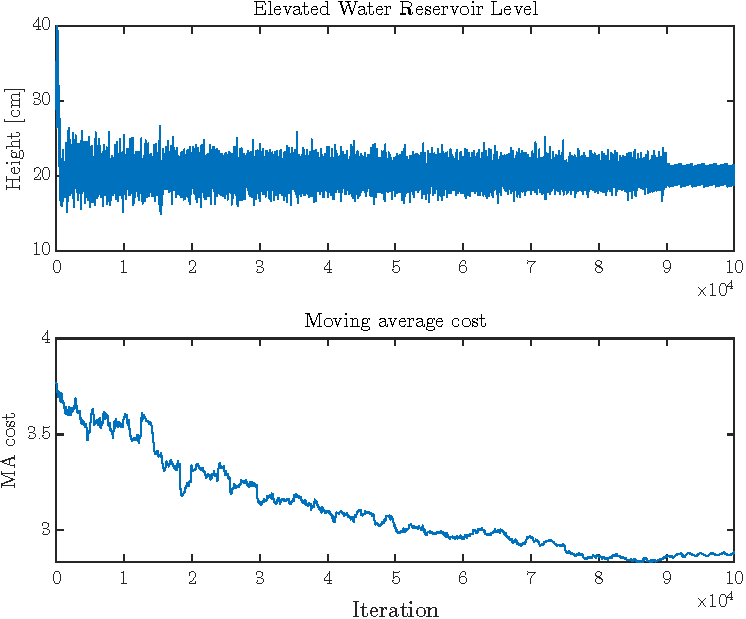
\includegraphics[width=0.7\linewidth]{figures/RemovedCenter.pdf}
	\caption{Continuous height results with feature near lower barrier removed.}
	\label{fig:RemovedCenter}
\end{figure}

\cref{fig:RemovedCenter} shows the results of removing the feature with center near the beginning of the lower barrier. The initial convergence now reaches much closer to the expected optimal height, but convergence in that area is much slower. Because points here are far away from any feature, their impact are weighted very low.

\begin{figure}[h!]
	\centering
	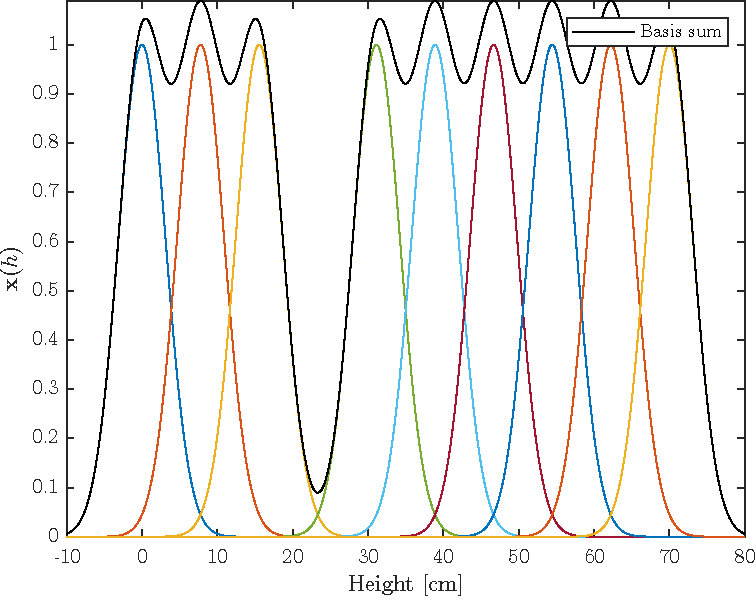
\includegraphics[width=0.7\linewidth]{figures/RemovedRBF.pdf}
	\caption{Radial basis functions with center near barrier removed.}
	\label{fig:RemovedRBF}
\end{figure}

\cref{fig:RemovedRBF} shows the radial basis functions with the barrier center removed. This clearly visualises the reason that overflow is reduced, but at the expense of having very little feature impact in that area causing learning to be very slow.

Another approach to removing the center, is to add more radial basis functions around the barrier beginning. This would cause the generalisation to be more accurate, meaning less overflow, without sacrificing learning.

Essentially, the number of radial basis functions, and placement of their centers can and should be included as a hyper parameter.


\section{Implicit Exploration}
Double approximation results showed very nice convergence without randomness. This is because we have implicit exploration from other elements. The oscillating demand very clearly results in a similar oscillation in states, this is seen in all water level plots. Initialisation of Q values and weights at 0, means whenever a cost is assigned to one action, all other actions are better until they have shown to yield even higher cost. The combination of these is very clear in the double approximation results \cref{fig:DoubleContResults1}, showing a very large range of states being explored before convergence.


\section{Generalisation to other Water Distribution Networks and Real World Implementation}
Here we present thought on the real life implementation of reinforcement learning. We have seen all method be quite sensitive to hyper parameters, and performance relies on demand balancing. We therefore doubt the method is easily applicable to all networks, some redesign and tuning will certainly be necessary. However, the laboratorie results are not performed without a finely tuned algorithm, and shows decent performance can be achieved with direct implementation. Finally, the tuning of a reinforcement learning is likely much less tedious than modelling a network, if it is even possible.

We have mentioned the minimisation of energy as a goal of this project. We cannot present evidence of this goal, but believe there is good reasoning to believe reinforcement learning can reduce energy usage. The algorithm clearly settles to a behaviour that it thinks is optimal. Whether this is actually optimal would require modelling of the system, and heavily depend on design of cost function and barriers. There is also the element of safe learning, the act of learning, without imposing dangerous states on the system. In this project the only indirect safety feature is imposed by the barrier function. Here we see the trade off between optimality and safety,  where the beginning of the lower barrier determines how low the algorithm settles, directly influencing the energy needed to satisfy demands.

Although approximation methods are showing safe learning, due to generalisation. We would not guarantee safety from these methods, before real implementation, methods to guarantee safe learning needs to be found, we would like to research this in future work. Further more, we remark the importance of demand balancing, which in real implementation can only realistically be done by carefully designing the pump setup, as demands cannot be controlled. 
